\documentclass[12pt, a4paper]{article}

\usepackage[utf8]{inputenc}
\usepackage[T1]{fontenc}
\usepackage[russian]{babel}
\usepackage[oglav,spisok,boldsect, figwhole]{./style/fn2kursstyle1}
\graphicspath{{./style/}{./figures/}}
\usepackage{float}%"Плавающие" картинки
\usepackage{multirow}
\usepackage{subcaption}
%Римские цифры
\newcommand{\RomanNumeralCaps}[1]
{\MakeUppercase{\romannumeral #1}}

\usepackage{comment}

%Параметры титульника
\title{Решение задач интерполирования}
\group{ФН2-52Б}
\author{Г.А.~Швецов}
\supervisor{А.О.~Гусев}
\date{2022}
\begin{document}
	\newcommand{\pl}{\partial}
	\maketitle
	
	\tableofcontents
	
	\newpage
	
	\section{Контрольные вопросы}
	% TODO %%%%%%%%%%%%%%%%%%%%%%%%%%%%%%%%%%%%%%%%%%%%%%%%%%%%
	\begin{enumerate}
		\item \textit{Определите количество арифметических операций, требуемое для интерполирования функции в некоторой точке
			многочленом Лагранжа (включая построение самого многочлена) на сетке с числом узлов, равным $n$.}
		\smallskip
		
		Многочлен Лагранжа имеет вид
		\begin{equation}
			L_n = \sum_{k = 0}^n y_k \prod_{j=0,\,j \ne k}^n \frac{x - x_j}{x_k - x_j}. 
			\label{first}
		\end{equation}
		
		
		Как видно из формулы (\ref{first}), в произведении мы имеем ровно $n$ делений и $n-1$ умножений. Каждое произведение мы домножаем на $y_k$ (1 умножение). В результате получаем $n+n-1+1=2n$ мультипликативных операций на каждом шаге. Просуммировав от $0$ до $n$, получаем $2n^2+2n$ арифметических операций. 
		\smallskip
		\item \textit{Определите количество арифметических операций, требуемое для интерполирования функции в некоторой точке
			кубическим сплайном (включая затраты на вычисление коэффициентов сплайна) на сетке с числом узлов, равным $n$}.
		\smallskip
		%		TODO 
		%		бинарный поиск не включен, думаю и не надо
		
		Для нахождения вспомогательного параметра $g_i$ необходимо $n$ делений. Для составления СЛАУ необходимо посчитать коэффициенты, требующие $2(n-1)$ умножений. Решаем СЛАУ методом прогонки, что требует $5n$ операций. Осталось заполнить оставшиеся коэффициенты. Это $5(n-1)+5=5n$ действий. Таким образом, для составления многочлена третьей степени необходимо затратить $n+2(n-1)+5n+5n=13n-2$ мультипликативных операций.
		
		Для интерполирования же функции в некоторой точке по формуле
		\begin{equation}
			s_i=a_i+b_i(x-x_{i-1})+c_i(x-x_{i-1})^2+d_i(x-x_{i-1})^3
			\label{second}
		\end{equation}
		требуется затратить еще 6 умножений. Итого $6+13n-2=13n+4$ операций.
		\smallskip
		\item \textit{Функция $f(x) = e^{x}$ интерполируется многочленом Лагранжа на отрезке $[0, 2]$ на равномерной сетке с шагом $h = 0,2$.
			Оцените ошибку экстраполяции в точке $x = 2{,}2$, построив многочлен Лагранжа и подставив в него это значение, а также по формуле для погрешности экстраполяции.}
		\smallskip
		
		Точка $x=2{,}2$ находится в интервале $x \in [b,b+h] = [2,\,2{,}2]$, поэтому оценим ошибку экстраполяции по следующей формуле
		\[
		|y(x)-L_n(x)|\le h^{n+1}\max_{\xi \in [a,\,x]}|y^{(n+1)}(\xi)|.
		\]
		В нашем же случае
		\[
		|y(x)-L_n(x)| = 6.2664084 \text{e-8} \le h^{n+1}\max_{\xi \in [a,\,x]}|y^{(n+1)}(\xi)| = 0.000000184832262.
		\]
		\item \textit{Выпишите уравнения для параметров кубического сплайна, если в узлах $x_0$ и $x_n$ помимо значений функции $y_0$ и $y_n$
			заданы первые производные $y'(x_0)$ и $y'(x_n)$.}
		\smallskip
		
		На каждом из отрезков $ [ x_{i - 1}, \, x_i ], \: i = \overline{1, \, n} $ функция $ S(x) = s_i(x) $ ищется  в виде многочлена третьей степени:
		\[
		s_i = a_i + b_i (x - x_{i - 1}) + c_i (x - x_{i - 1})^2 + d_i (x - x_{i - 1})^3. 
		\]
		Найдем коэффициенты $ a_i, \, b_i, \, c_i, \, d_i $. Т.к. $ S(x_i) = y_i, \: i = \overline{0, \, n} $ получим:			
		\begin{gather*}
			a_i = y_{i - 1}, i = \overline{1, \, n}, \\
			a_i + b_i h_i + c_i h_i^2 + d_i h_i^3 = y_i, \: i = \overline{1, \, n}.
		\end{gather*}
		Здесь $ h_i = x_i - x_{i - 1} $ --- длина отрезка $[x_{i-1},x_i]$. 
		
		Из условия непрерывности первой и второй производной для внутренних узлов сетки получим:
		\begin{gather*}
			\begin{aligned}
				S'(x_i - 0) &= S'(x_i + 0), \\
				S''(x_i - 0) &= S''(x_i + 0), \: i = \overline{1, \, (n - 1)},
			\end{aligned}
		\end{gather*}
		откуда:
		\begin{gather*}
			b_i + 2 c_i h_i + 3 d_i h_i^2 = b_{i + 1}, \: i = \overline{1, \, (n - 1)}, \\
			2 c_i + 6d_i h_i = 2 c_{i + 1}, \: i = \overline{1, \, (n - 1)}.
		\end{gather*}
		Получаем систему из $ (4 n - 2) $ уравнений с $ 4 n $ неизвестными.
		Недостающие два уравнения получим из граничных условий для $S(x)$:
		\[
		S'(x_0) = y_0', \qquad S'(x_n) = y_n'. 
		\]
		Получим
		\begin{gather*}
			S'(x_0) = s_1'(x_0) =  b_1 = y'(x_0), \\
			S'(x_n) = s_n'(x_n) = b_n + 2 c_n h_n + 3 d_n h_n^2 = y'(x_n).
		\end{gather*}
		
		Выражения для коэффициентов $ b_i $ и $ d_i $ имеют вид
		
		\begin{gather*}
			\begin{aligned}
				b_i &= g_i - \frac{(c_{i + 1} + 2 c_i) h_i}{3}, \\
				d_i &= \frac{c_{i + 1} -c_i}{3 h_i}, \: i = \overline{1, \, n},
			\end{aligned}
		\end{gather*}
		где $ g_i = \dfrac{y_i - y_{i - 1}}{h_i} $.
		
		Тогда граничные условия для $ S(x) $ можно переписать в следующем виде:
		\begin{gather*}
			\begin{aligned}
				c_1 &= \frac{3 (g_1 - y_0')}{2 h_1} - \frac{c_2}{2}, \\
				c_{n + 1} &= \frac{3 (y_n' - g_n)}{2 h_n} - \frac{c_n}{2}.
			\end{aligned}
		\end{gather*}
		
		Тогда, исключая из предыдущих уравнений переменные $ a_i, \, b_i, \, d_i $, получим систему
		\begin{equation*}
			\left\{
			\begin{aligned}
				&c_1 = \frac{3 (g_1 - y_0')}{2 h_1} - \frac{c_2}{2}, \\
				&h_{i - 1} c_{i - 1} + 2 (h_{i - 1} + h_i) c_i + h_i c_{i + 1} = 3 (g_i - g_{i - 1}),  \: i = \overline{2, \, n}. \\
				&c_{n + 1} = \frac{3 (y_n' - g_n)}{2 h_n} - \frac{c_n}{2}.
			\end{aligned}
			\right.
		\end{equation*}
		\smallskip
		
		\item \textit{Каковы достоинства и недостатки сплайн-интерполяции
			и интерполяции многочленом Лагранжа?}
		\smallskip
		
		\textbf{Интерполяция многочленом Лагранжа}
		
		
		Достоинства:
		\begin{enumerate}
			\item Построенная функция имеет непрерывные производные любого порядка;
		\end{enumerate}
		Недостатки:
		\begin{enumerate}
			\item Интерполирование функции при большом числе узлов интерполяции приводит к плохому приближению;
			\item Рост погрешности округления;
			\item По сравнению со сплайн-интерполяцией сложность алгоритма на порядок выше ($O(n^2)$);
			\item При добавлении новых узлов интерполяции, многочлен Лагранжа требуется заново строить;
			\item Применение многочленов высоких степеней приводит к осцилляциям (пример Рунге). 
		\end{enumerate}
		
		\newpage
		\textbf{Сплайн-интерполяция}
		
		Достоинства:
		\begin{enumerate}
			\item Степень многочленов не зависит от числа узлов сетки и, следовательно, не изменяется при его увеличении;
			\item Построенная функция имеет $(p-1)$ непрерывных производных;
			% Из методички
			\item В случае интерполяции кубическими сплайнами не только сам сплайн $S(x)$, но и его первая и вторая производные $S'(x)$ и $S''(x)$ также сходятся в равномерной норме к соответствующим производным функциям $y(x)$.
		\end{enumerate}
		Недостатки:
		\begin{enumerate}
			\item Большая вероятность, что экстраполяция функции приведет к большой ошибке.
		\end{enumerate}
		\smallskip
		\item \textit{Какие свойства полиномов Чебышева и чебышевских сеток Вам известны?}
		\smallskip
		
		При проведении интерполяции желательно, чтобы была достигнута минимальная ошибка $\|f-\tilde{f}\|$ в некоторой норме.
		\begin{equation}
			\|f-\tilde{f}\|_C=\|r_n\|_C \le \frac{M_{n+1}}{(n+1)!}\|\omega\|_C.
			\label{grade}
		\end{equation}
		Поэтому выбирают такой набор узлов, чтобы норма в правой части оценки (\ref{grade}) была минимальной, тем самым уменьшая ошибку интерполяции
		\[
		\min_{x_0,\dots,x_n} \max_{[a,b]}|\omega(x)|,\quad
		\omega(x) = \prod_{i=0}^{n}(x-x_i).
		\]
		Это задача о построении полинома $(n+1)$-го порядка, которая решена В.А.~Марковым. Искомый полином является полиномом Чебышева первого рода и имеет вид
		\[
		\omega(x)=T_{n+1}(x) = \frac{(b-a)^{n+1}}{2^{2n+1}}\cos\left((n+1)\arccos\frac{2x-(b+a)}{b-a}\right),
		\]
		корни полинома задаются следующим соотношением:
		\[
		x_k=\frac{a+b}{2}+\frac{b-a}{2}\cos\frac{(2k+1)\pi}{2(n+1)},\quad k=0,\,1,\dots,\,n,
		\]
		при этом они являются узлами интерполяции. Для такого набора узлов
		\[
		\|\omega\|_C=\frac{1}{2^{2n+1}}(b-a)^{n+1}
		\]
		и
		\[
		\|f-L_n\|_C \le \frac{M_{n+1}}{(n+1)!}\frac{(b-a)^{n+1}}{2^{2n+1}}.
		\]
		Полученная оценка является неулучшаемой. 
	\end{enumerate}
	\newpage
	\section{Результаты}
	
	\begin{figure}[H]
		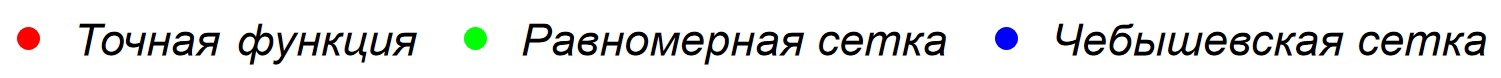
\includegraphics[width=\textwidth]{labels}
	\end{figure}
	
	
	\subsection{Функция $x$}
	
	\begin{table}[H]
		\caption{Нормы ошибок интерполяции.}
		\centering
		\footnotesize
		\begin{tabular}{|c|c|c|c|c|}
			\hline
			\multirow{2}{5em}{Количество узлов} & \multicolumn{2}{|c|}{Интерполирование многочленом Лагранжа}&\multicolumn{2}{|c|}{Сплайн-интерполирование}\\
			\cline{2-5}
			&Равномерная сетка &Чебышевская сетка &Равномерная сетка&Чебышевская сетка\\
			\hline
			4& 0.00000000&0.00000000&0.00000000&0.00000000\\
			\hline
			8&0.00000000&0.00000000&0.00000000&0.00000000\\
			\hline
			16&0.00000000&0.00000000&0.00000000& 0.00000000\\
			\hline
			32&0.00000000&0.00000000&0.00000000&0.00000000\\
			\hline
			64&0.00000000&0.00000000&0.00000000&0.00000000\\
			\hline
		\end{tabular}
	\end{table}
	
	
	\begin{figure}[H]
		\centering
		\begin{subfigure}{0.4\textwidth}
			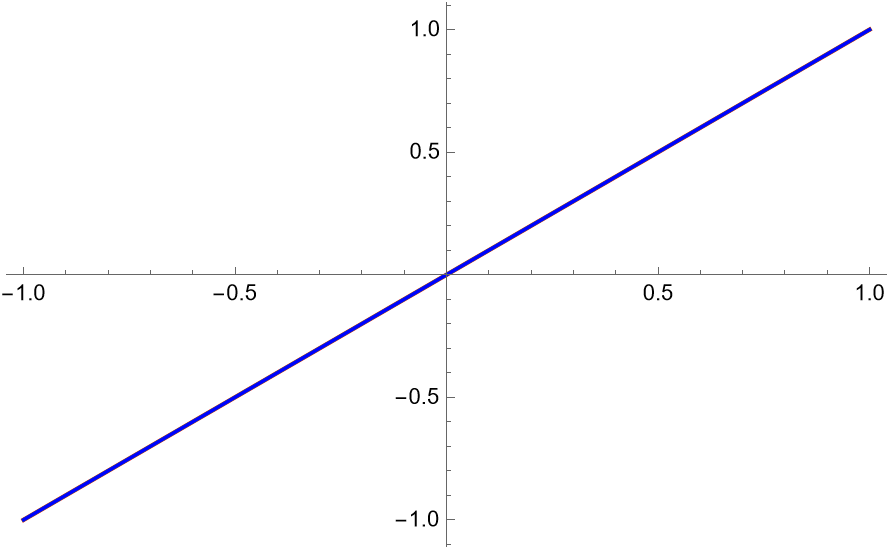
\includegraphics[width=\textwidth]{1_l8}
			\caption{Интерполяция многочленом Лагранжа}
		\end{subfigure}
		\hfill
		\begin{subfigure}{0.4\textwidth}
			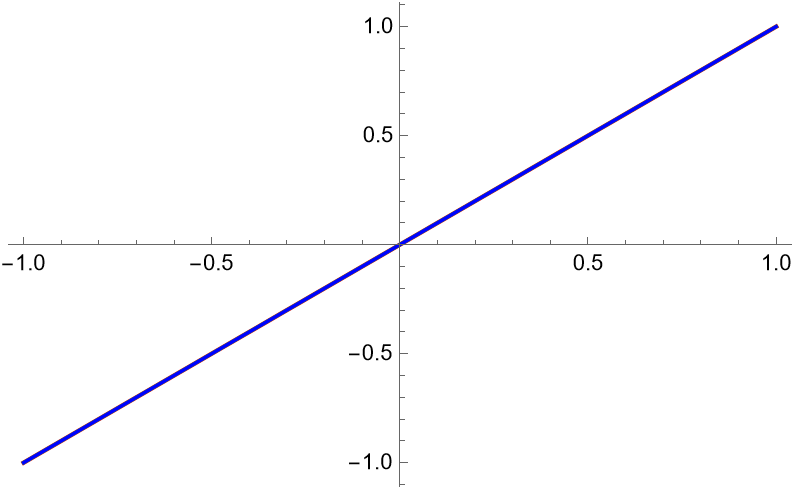
\includegraphics[width=\textwidth]{1_s8}
			\caption{Сплайн-интерполяция}
		\end{subfigure}
		\hfill
		\\[0.5cm]
		\caption{$n = 8$.}
		\label{fig:figures}
	\end{figure}
	
	
	\subsection{Функция $x^2$}
	
	\begin{table}[H]
		\caption{Нормы ошибок интерполяции.}
		\centering
		\footnotesize
		\begin{tabular}{|c|c|c|c|c|}
			\hline
			\multirow{2}{5em}{Количество узлов} & \multicolumn{2}{|c|}{Интерполирование многочленом Лагранжа}&\multicolumn{2}{|c|}{Сплайн-интерполирование}\\
			\cline{2-5}
			&Равномерная сетка &Чебышевская сетка &Равномерная сетка&Чебышевская сетка\\
			\hline
			4& 0.00000000&0.00000000&0.02406589&0.01356303\\
			\hline
			8&0.00000000&0.00000000&0.00613592&0.00150945\\
			\hline
			16&0.00000000&0.00000000&0.00153414& 0.00012378\\
			\hline
			32&0.00000000&0.00000000&0.00038353&0.00000882\\
			\hline
			64&0.23398295&0.00000000&0.00000000&0.00000000\\
			\hline
		\end{tabular}
	\end{table}
	
	
	\begin{figure}[H]
		\centering
		\begin{subfigure}{0.4\textwidth}
			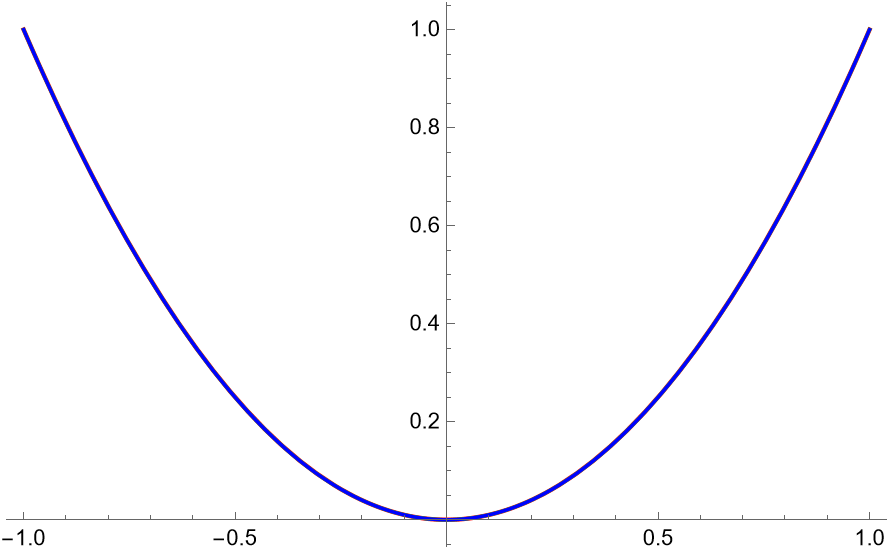
\includegraphics[width=\textwidth]{1_l4}
			\caption{Интерполяция многочленом Лагранжа}
		\end{subfigure}
		\hfill
		\begin{subfigure}{0.4\textwidth}
			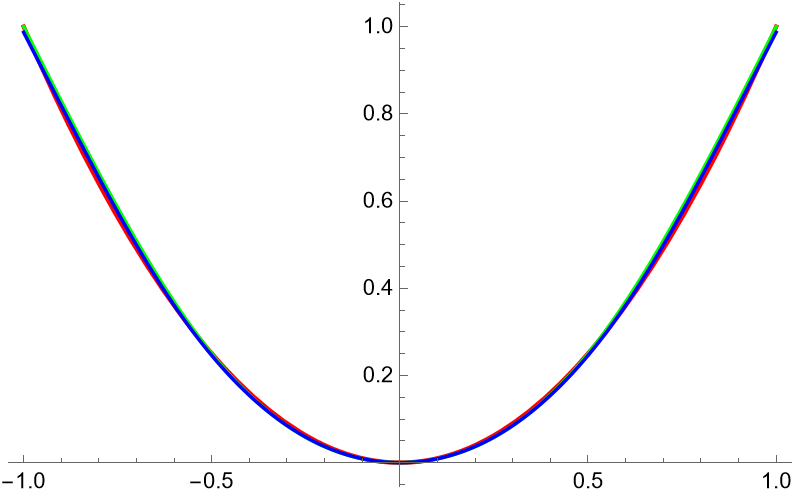
\includegraphics[width=\textwidth]{1_s4}
			\caption{Сплайн-интерполяция}
		\end{subfigure}
		\hfill
		\\[0.5cm]
		\caption{$n = 4$.}
	\end{figure}
	
	\begin{figure}[H]
		\centering
		\begin{subfigure}{0.4\textwidth}
			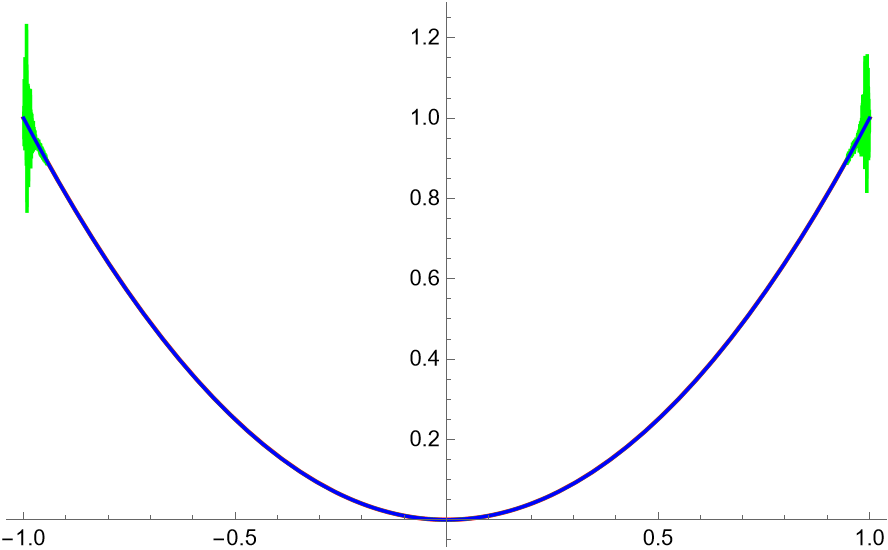
\includegraphics[width=\textwidth]{1_l64}
			\caption{Интерполяция многочленом Лагранжа}
		\end{subfigure}
		\hfill
		\begin{subfigure}{0.4\textwidth}
			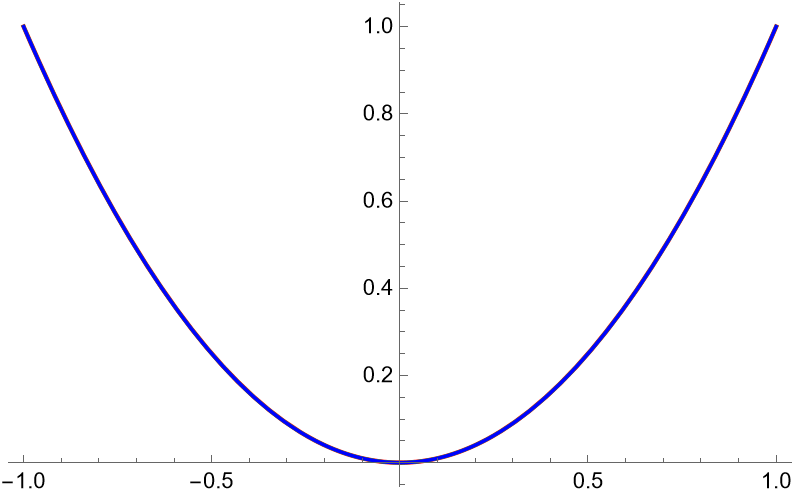
\includegraphics[width=\textwidth]{1_s64}
			\caption{Сплайн-интерполяция}
		\end{subfigure}
		\hfill
		\\[0.5cm]
		\caption{$n = 64$.}
	\end{figure}
	
	
	\begin{table}[H]
		\caption{Нормы ошибок интерполяции.}
		\centering
		\footnotesize
		\begin{tabular}{|c|c|c|c|c|}
			\hline
			\multirow{2}{5em}{Количество узлов} & \multicolumn{2}{|c|}{Интерполирование многочленом Лагранжа}&\multicolumn{2}{|c|}{Сплайн-интерполирование}\\
			\cline{2-5}
			&Равномерная сетка &Чебышевская сетка &Равномерная сетка&Чебышевская сетка\\
			\hline
			100& 749213958068.13720703&0.00000000&0.00000000&0.00000000\\
			\hline
		\end{tabular}
	\end{table}
	
	
	\begin{figure}[H]
		\centering
		\begin{subfigure}{0.4\textwidth}
			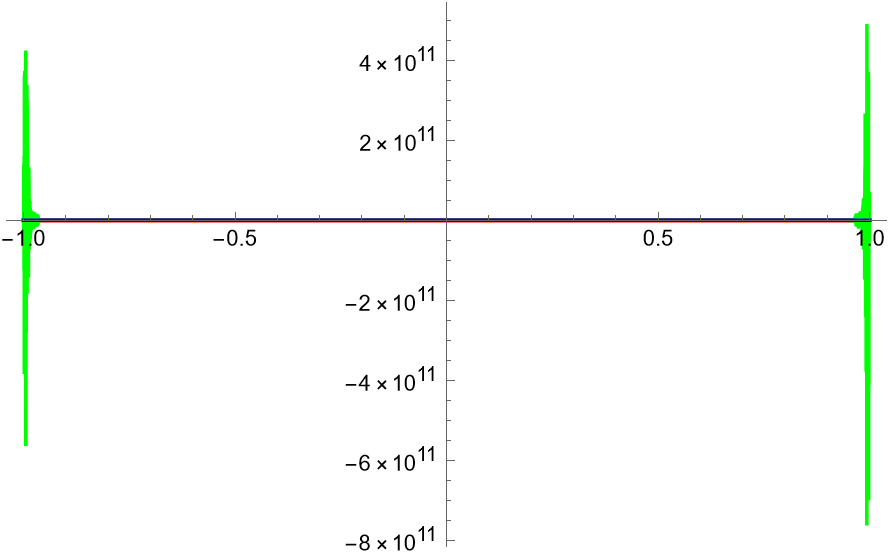
\includegraphics[width=\textwidth]{0_l100}
			\caption{Интерполяция многочленом Лагранжа}
		\end{subfigure}
		\hfill
		\begin{subfigure}{0.4\textwidth}
			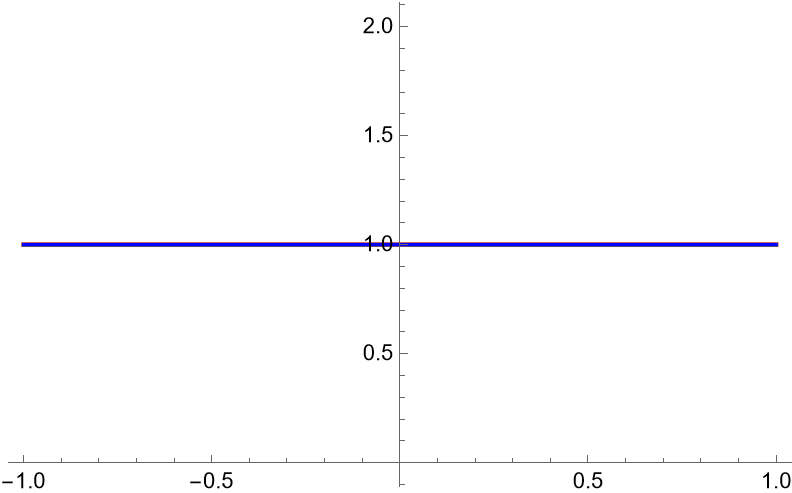
\includegraphics[width=\textwidth]{0_s100}
			\caption{Сплайн-интерполяция}
		\end{subfigure}
		\hfill
		\\[0.5cm]
		\caption{$n = 100$.}
	\end{figure}
	
	
	\begin{table}[H]
		%	\caption{Нормы ошибок интерполяции.}
		\centering
		\footnotesize
		\begin{tabular}{|c|c|c|c|c|}
			\hline
			\multirow{2}{5em}{Количество узлов} & \multicolumn{2}{|c|}{Интерполирование многочленом Лагранжа}&\multicolumn{2}{|c|}{Сплайн-интерполирование}\\
			\cline{2-5}
			&Равномерная сетка &Чебышевская сетка &Равномерная сетка&Чебышевская сетка\\
			\hline
			4& 0.14720062&0.12317574&0.08583173&0.09777330\\
			\hline
			8& 0.31575341&0.06697527&0.04251731&0.05758552\\
			\hline
			16& 11.13706900&0.03520988&0.02125762&0.03116576\\
			\hline
		\end{tabular}
	\end{table}
	
	
	\begin{figure}[H]
		\centering
		\begin{subfigure}{0.4\textwidth}
			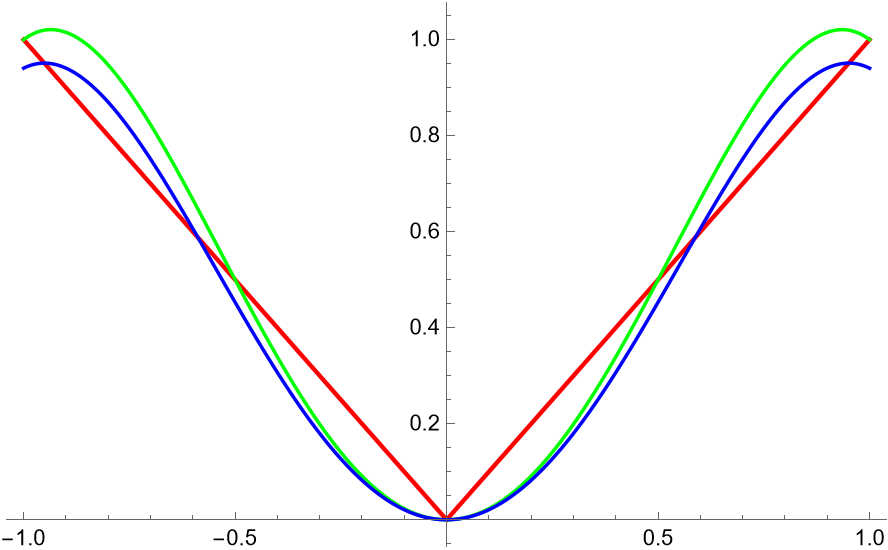
\includegraphics[width=\textwidth]{7_l4}
			\caption{Интерполяция многочленом Лагранжа}
		\end{subfigure}
		\hfill
		\begin{subfigure}{0.4\textwidth}
			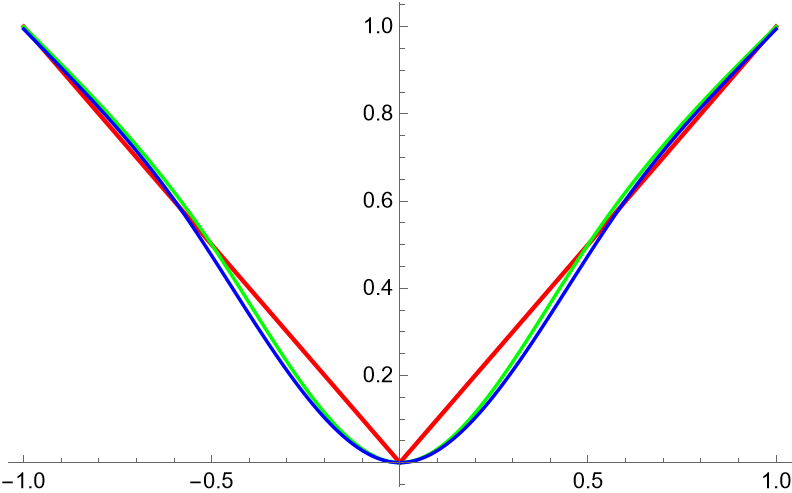
\includegraphics[width=\textwidth]{7_s4}
			\caption{Сплайн-интерполяция}
		\end{subfigure}
		\hfill
		\\[0.5cm]
		\caption{$n = 4$.}
	\end{figure}
	
	\begin{figure}[H]
		\centering
		\begin{subfigure}{0.4\textwidth}
			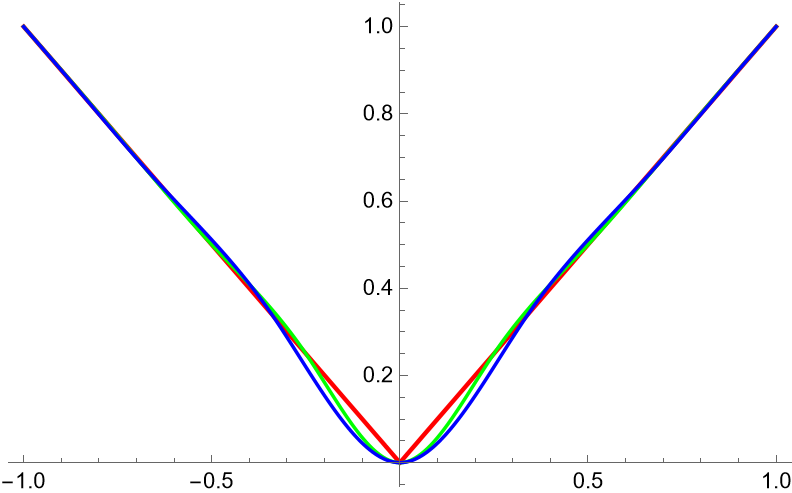
\includegraphics[width=\textwidth]{7_s8}
			\caption{Сплайн-интерполяция ($n=8$)}
		\end{subfigure}
		\hfill
		\begin{subfigure}{0.4\textwidth}
			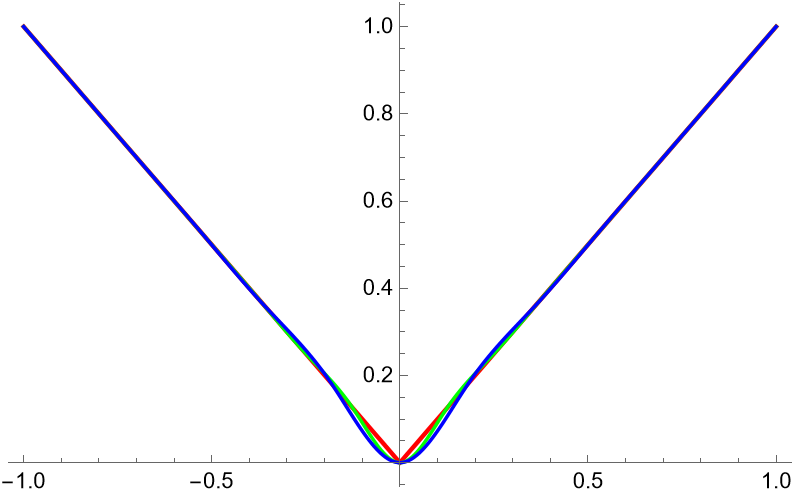
\includegraphics[width=\textwidth]{7_s16}
			\caption{Сплайн-интерполяция ($n=16$)}
		\end{subfigure}
		\hfill
		\\[0.5cm]
		\caption{$n = 8$.}
	\end{figure}
	
	
	
	\newpage
	\subsection{Функция $\sfrac{1}{\arcctg{(1+10 x^2)}}$}
	
	\begin{table}[H]
		\caption{Нормы ошибок интерполяции.}
		\centering
		\footnotesize
		\begin{tabular}{|c|c|c|c|c|}
			\hline
			\multirow{2}{5em}{Количество узлов} & \multicolumn{2}{|c|}{Интерполирование многочленом Лагранжа}&\multicolumn{2}{|c|}{Сплайн-интерполирование}\\
			\cline{2-5}
			&Равномерная сетка &Чебышевская сетка &Равномерная сетка&Чебышевская сетка\\
			\hline
			4& 0.41874070&0.43984510&0.37888740&0.40442884\\
			\hline
			8&1.24549676&0.31118342&0.20291020&0.28341571\\
			\hline
			16&54.25190820&0.14203880&0.04443190& 0.12179101\\
			\hline
			32&194964.99928579&0.02735275&0.00297114&0.01344388\\
			\hline
			64&3255214956736.39648438&0.00108219&0.00049753&0.00236323\\
			\hline
		\end{tabular}
	\end{table}
	
	\begin{figure}[H]
		\centering
		\begin{subfigure}{0.4\textwidth}
			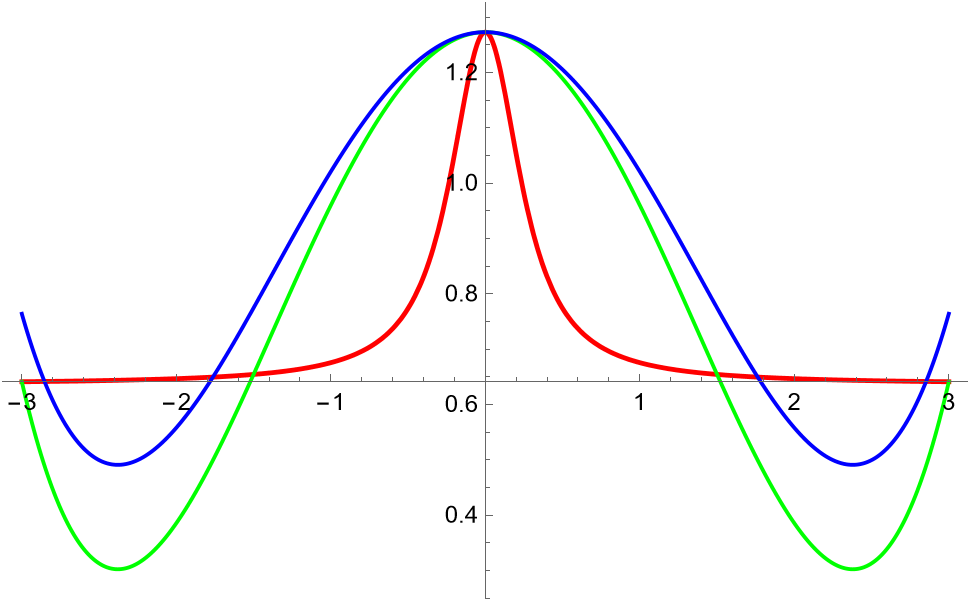
\includegraphics[width=\textwidth]{3_l4}
			\caption{Интерполяция многочленом Лагранжа}
		\end{subfigure}
		\hfill
		\begin{subfigure}{0.4\textwidth}
			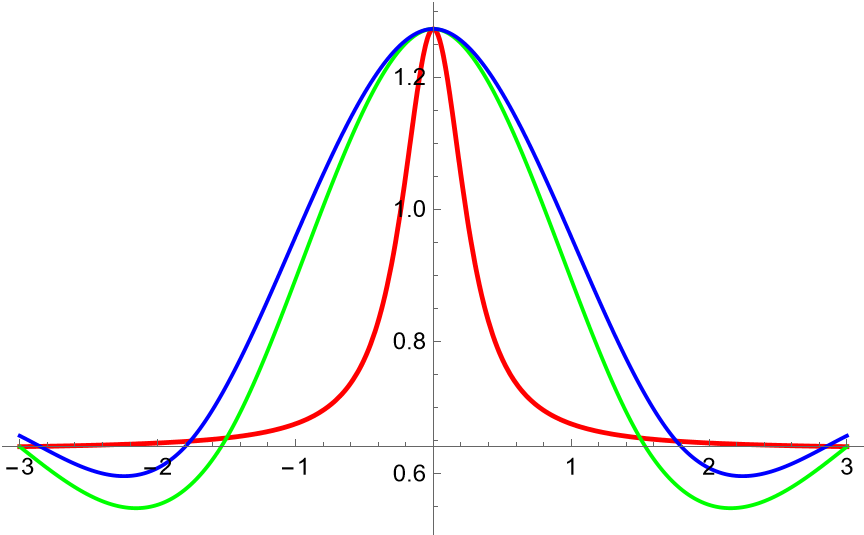
\includegraphics[width=\textwidth]{3_s4}
			\caption{Сплайн-интерполяция}
		\end{subfigure}
		\hfill
		\\[0.5cm]
		\caption{$n = 4$.}
		\label{fig:figures}
	\end{figure}
	
	\begin{figure}[H]
		\centering
		\begin{subfigure}{0.4\textwidth}
			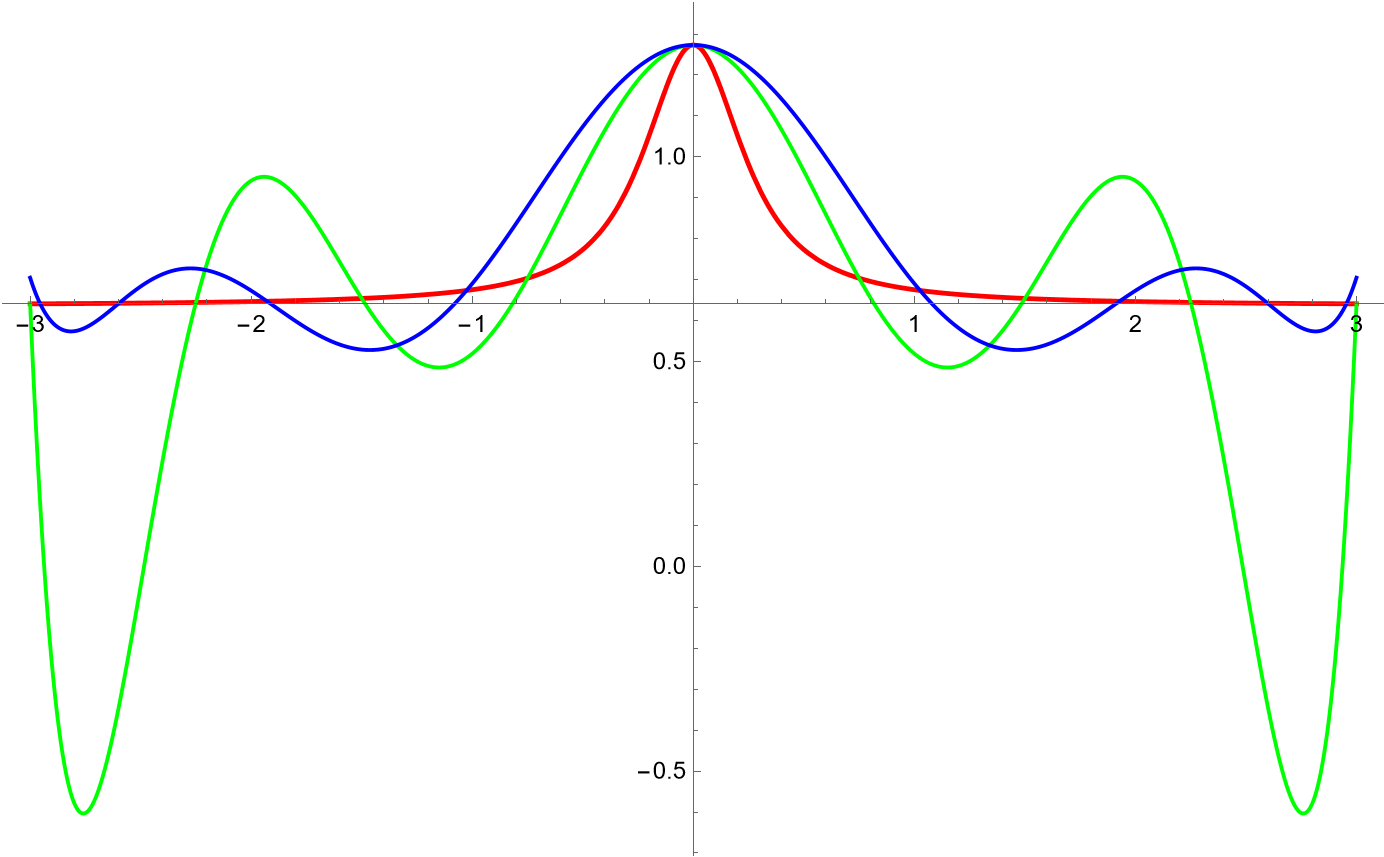
\includegraphics[width=\textwidth]{3_l8}
			\caption{Интерполяция многочленом Лагранжа}
		\end{subfigure}
		\hfill
		\begin{subfigure}{0.4\textwidth}
			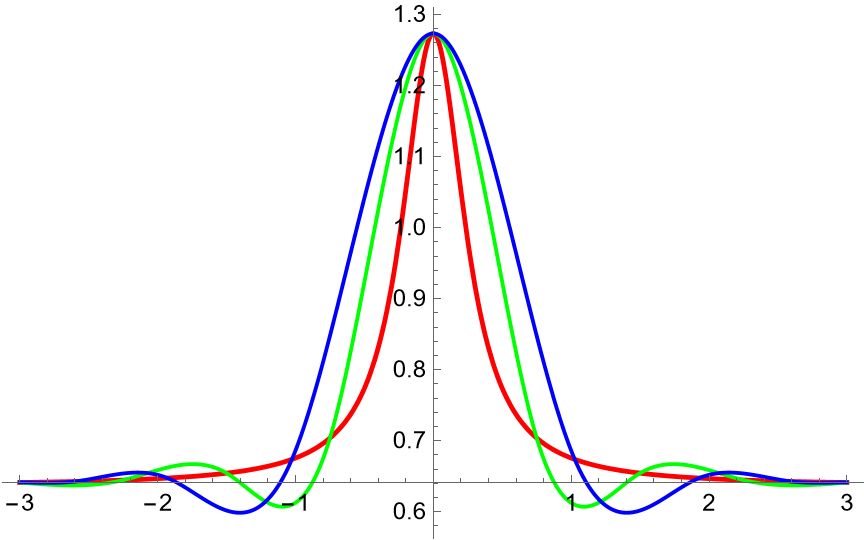
\includegraphics[width=\textwidth]{3_s8}
			\caption{Сплайн-интерполяция}
		\end{subfigure}
		\hfill
		\\[0.5cm]
		\caption{$n = 8$.}
		\label{fig:figures}
	\end{figure}
	
	
	\subsection{Функция $\sfrac{1}{1+x^2}$}
	
	\begin{table}[H]
		\caption{Нормы ошибок интерполяции.}
		\centering
		\footnotesize
		\begin{tabular}{|c|c|c|c|c|}
			\hline
			\multirow{2}{5em}{Количество узлов} & \multicolumn{2}{|c|}{Интерполирование многочленом Лагранжа}&\multicolumn{2}{|c|}{Сплайн-интерполирование}\\
			\cline{2-5}
			&Равномерная сетка &Чебышевская сетка &Равномерная сетка&Чебышевская сетка\\
			\hline
			4& 0.02228186&0.01219512&0.01027558&0.00448152\\
			\hline
			8&0.00225838&0.00035894&0.00162533&0.00085716\\
			\hline
			16&0.00003991&0.00000031&0.00038882& 0.00007959\\
			\hline
			32&0.00000003&0.00000000&0.00009620&0.00000530\\
			\hline
			64&16.96613580&0.00000000&0.00002399&0.00000034\\
			\hline
		\end{tabular}
	\end{table}
	
	\begin{figure}[H]
		\centering
		\begin{subfigure}{0.4\textwidth}
			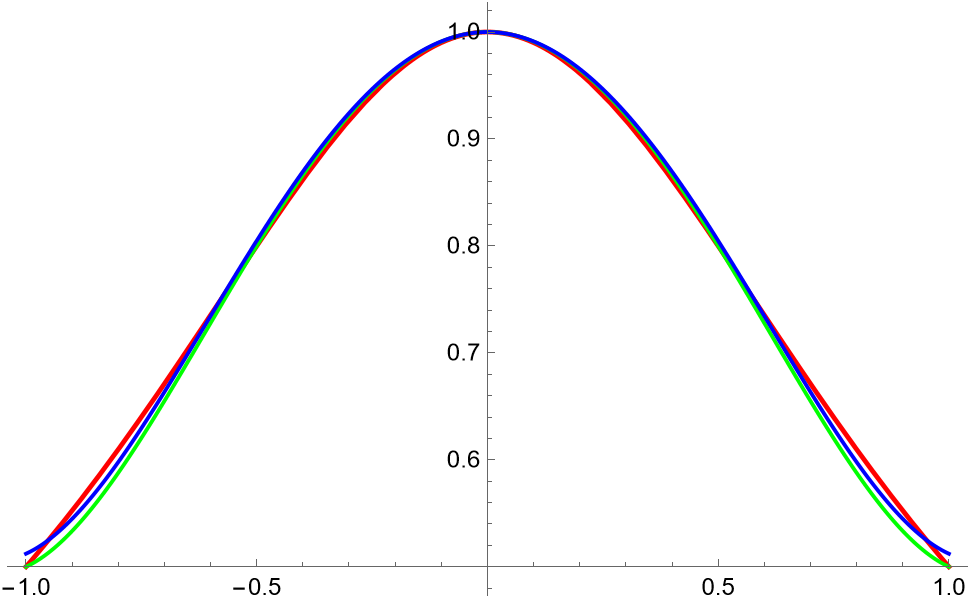
\includegraphics[width=\textwidth]{2_l4}
			\caption{Интерполяция многочленом Лагранжа}
		\end{subfigure}
		\hfill
		\begin{subfigure}{0.4\textwidth}
			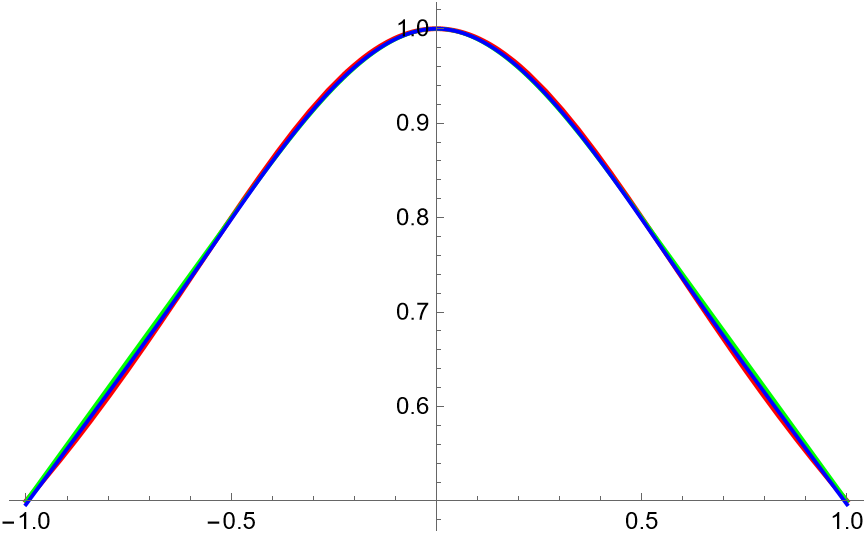
\includegraphics[width=\textwidth]{2_s4}
			\caption{Сплайн-интерполяция}
		\end{subfigure}
		\hfill
		\\[0.5cm]
		\caption{$n = 4$.}
	\end{figure}
	
	
	\begin{figure}[H]
		\centering
		\begin{subfigure}{0.4\textwidth}
			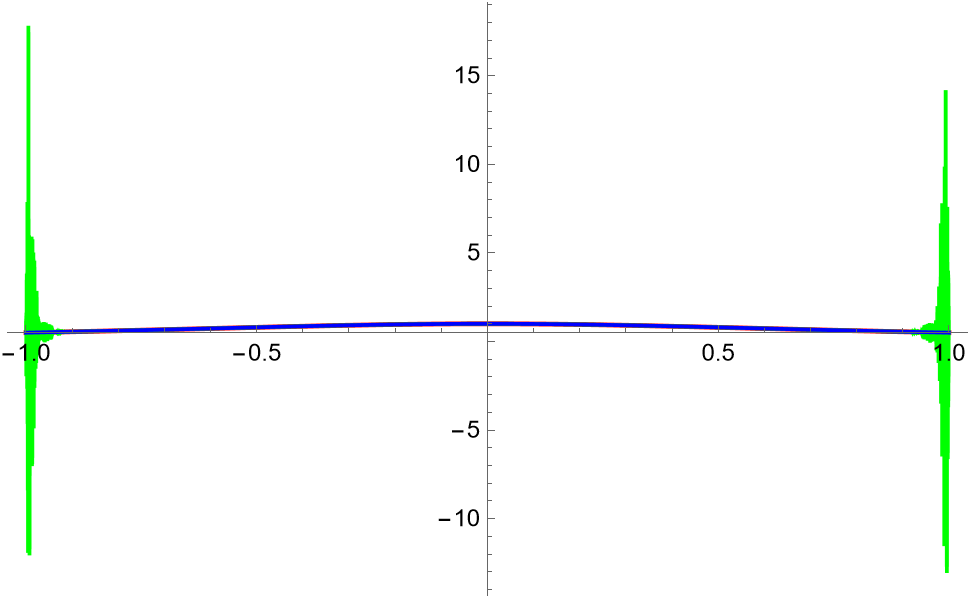
\includegraphics[width=\textwidth]{2_l64}
			\caption{Интерполяция многочленом Лагранжа}
		\end{subfigure}
		\hfill
		\begin{subfigure}{0.4\textwidth}
			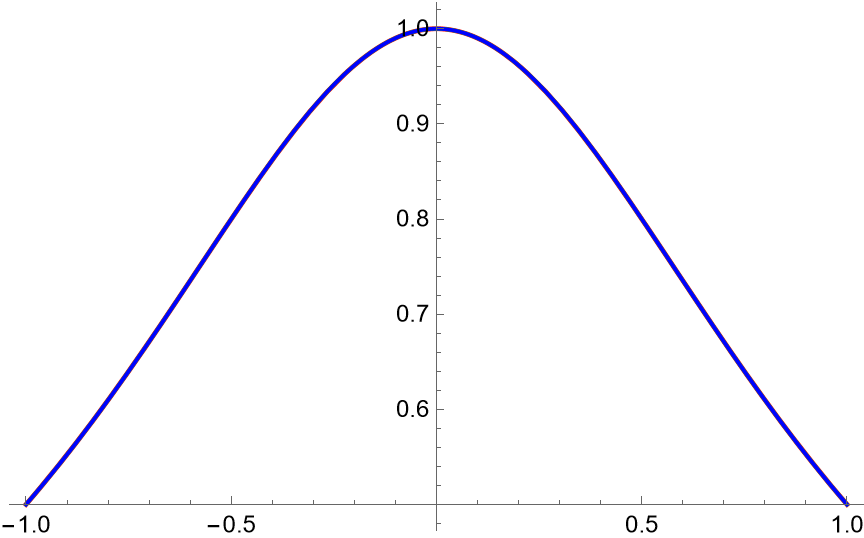
\includegraphics[width=\textwidth]{2_s64}
			\caption{Сплайн-интерполяция}
		\end{subfigure}
		\hfill
		\\[0.5cm]
		\caption{$n = 64$.}
	\end{figure}
	
	\subsection{Функция $\sfrac{1}{1+25x^2}$}
	
	\begin{table}[H]
		\caption{Нормы ошибок интерполяции.}
		\centering
		\footnotesize
		\begin{tabular}{|c|c|c|c|c|}
			\hline
			\multirow{2}{5em}{Количество узлов} & \multicolumn{2}{|c|}{Интерполирование многочленом Лагранжа}&\multicolumn{2}{|c|}{Сплайн-интерполирование}\\
			\cline{2-5}
			&Равномерная сетка &Чебышевская сетка &Равномерная сетка&Чебышевская сетка\\
			\hline
			4&0.43835712&0.40201690&0.27931341&0.33008954\\
			\hline
			8&1.04517650&0.17083545&0.05607385&0.13375079\\
			\hline
			16&14.39385129& 0.03261358&0.00374540&0.01362665\\
			\hline
			32&5058.95984109&0.00140174&0.0006555&0.00275683\\
			\hline
			64&1078549277.25717545&0.00000245&0.00004034&0.00024212\\
			\hline
			
		\end{tabular}
	\end{table}
	
	
	\begin{figure}[H]
		\centering
		\begin{subfigure}{0.4\textwidth}
			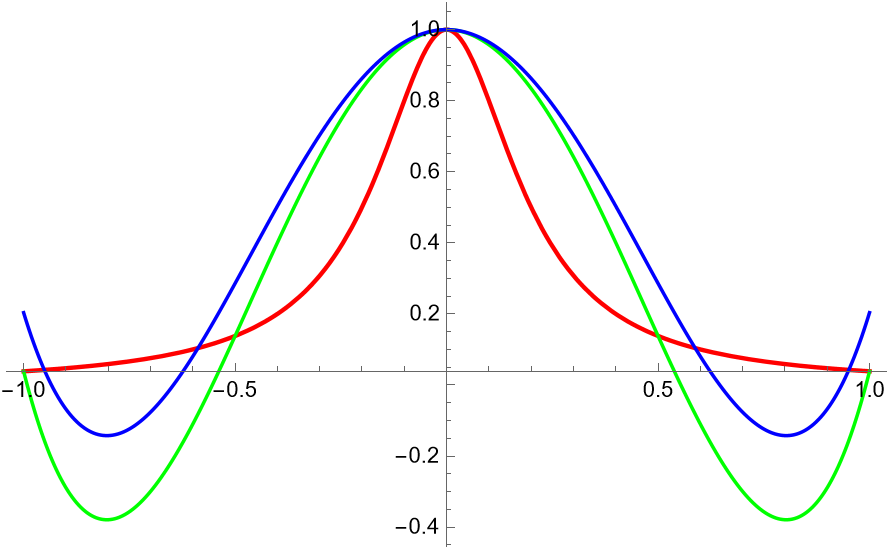
\includegraphics[width=\textwidth]{5_l4}
			\caption{Интерполяция многочленом Лагранжа}
		\end{subfigure}
		\hfill
		\begin{subfigure}{0.4\textwidth}
			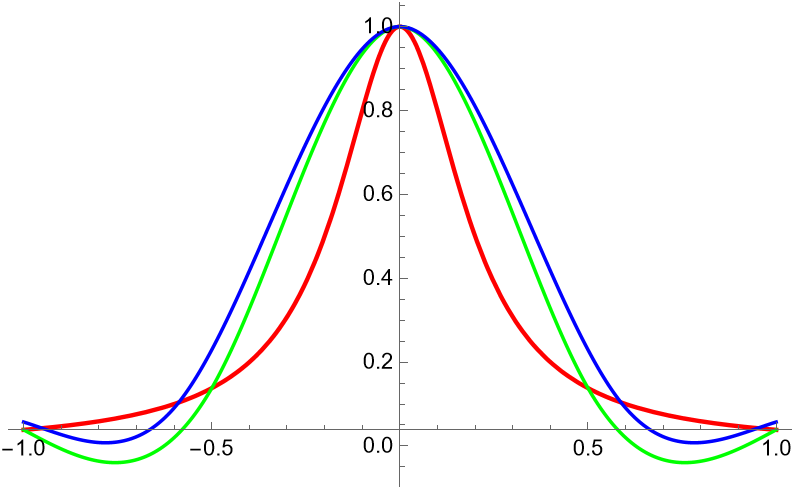
\includegraphics[width=\textwidth]{5_s4}
			\caption{Сплайн-интерполяция}
		\end{subfigure}
		\hfill
		\\[0.5cm]
		\caption{$n=4$.}
	\end{figure}
	
	
	\hfill
	
	\begin{figure}[H]
		\centering
		\begin{subfigure}{0.4\textwidth}
			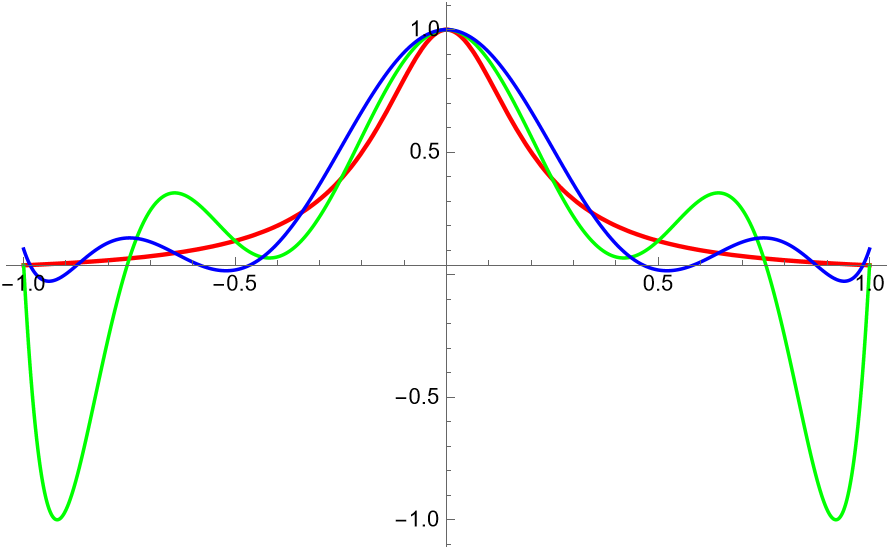
\includegraphics[width=\textwidth]{5_l8}
			\caption{Интерполяция многочленом Лагранжа}
		\end{subfigure}
		\hfill
		\begin{subfigure}{0.4\textwidth}
			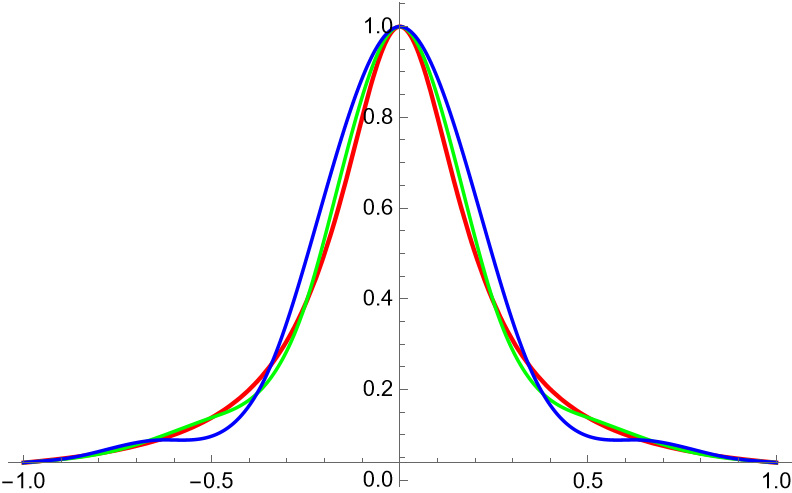
\includegraphics[width=\textwidth]{5_s8}
			\caption{Сплайн-интерполяция}
		\end{subfigure}
		\hfill
		\\[0.5cm]
		\caption{$n=8$.}
	\end{figure}
	
	\subsection{Функция $(4 x^3+2 x^2-4x+2)^{\sqrt 2} +\arcsin{\left(\sfrac{1}{5+x-x^2}\right)}-5$}
	
	\begin{table}[H]
		\caption{Нормы ошибок интерполяции.}
		\centering
		\footnotesize
		\begin{tabular}{|c|c|c|c|c|}
			\hline
			\multirow{2}{5em}{Количество узлов} & \multicolumn{2}{|c|}{Интерполирование многочленом Лагранжа}&\multicolumn{2}{|c|}{Сплайн-интерполирование}\\
			\cline{2-5}
			&Равномерная сетка &Чебышевская сетка &Равномерная сетка&Чебышевская сетка\\
			\hline
			4&0.59961429&0.33079347&1.15371582&0.63506019\\
			\hline
			8&0.02477320&0.00794910&0.32412950&0.07820568\\
			\hline
			16&0.00853480&0.00007259&0.08226211&0.00660738\\
			\hline
			32&0.00321827&0.00000003&0.02065464&0.00047461\\
			\hline
			64&33.93813773&0.00000000&0.00516903&0.00003170\\
			\hline
		\end{tabular}
	\end{table}
	
	
	\begin{figure}[H]
		\centering
		\begin{subfigure}{0.4\textwidth}
			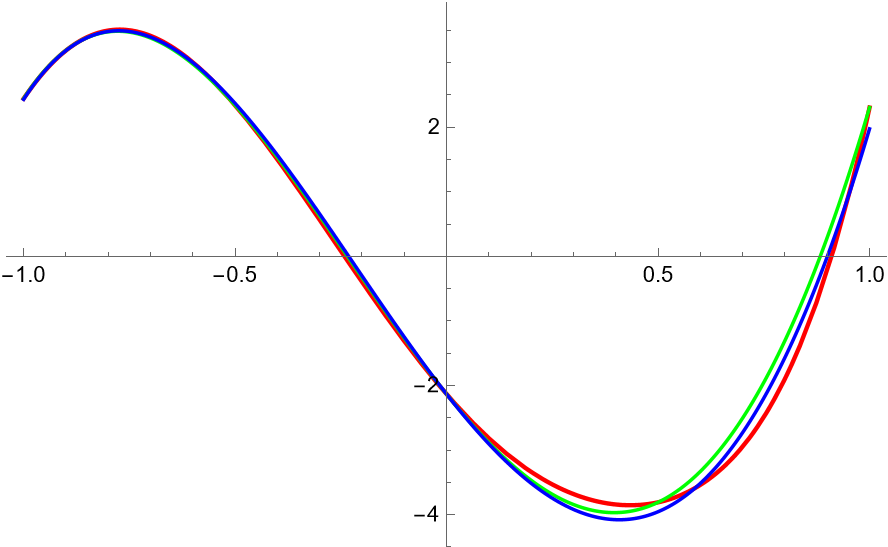
\includegraphics[width=\textwidth]{4_l4}
			\caption{Интерполяция многочленом Лагранжа}
		\end{subfigure}
		\hfill
		\begin{subfigure}{0.4\textwidth}
			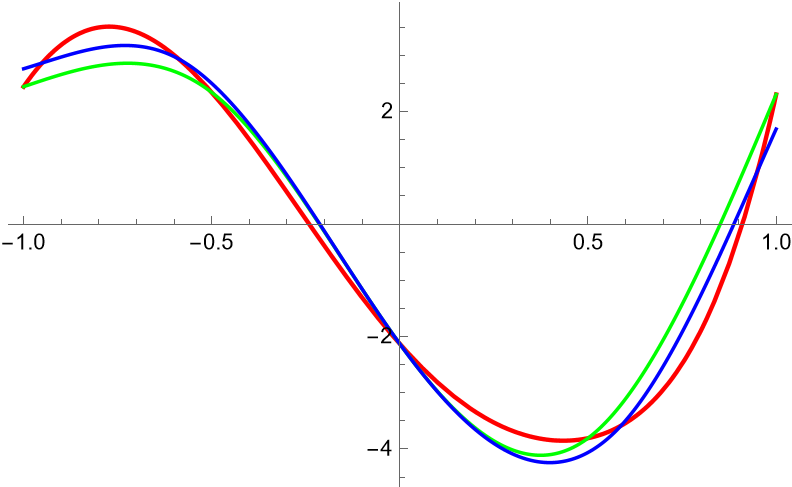
\includegraphics[width=\textwidth]{4_s4}
			\caption{Сплайн-интерполяция}
		\end{subfigure}
		\hfill
		\\[0.5cm]
		\caption{$n = 4$.}
	\end{figure}
	
	\hfill
	
	\begin{figure}[H]
		\centering
		\begin{subfigure}{0.4\textwidth}
			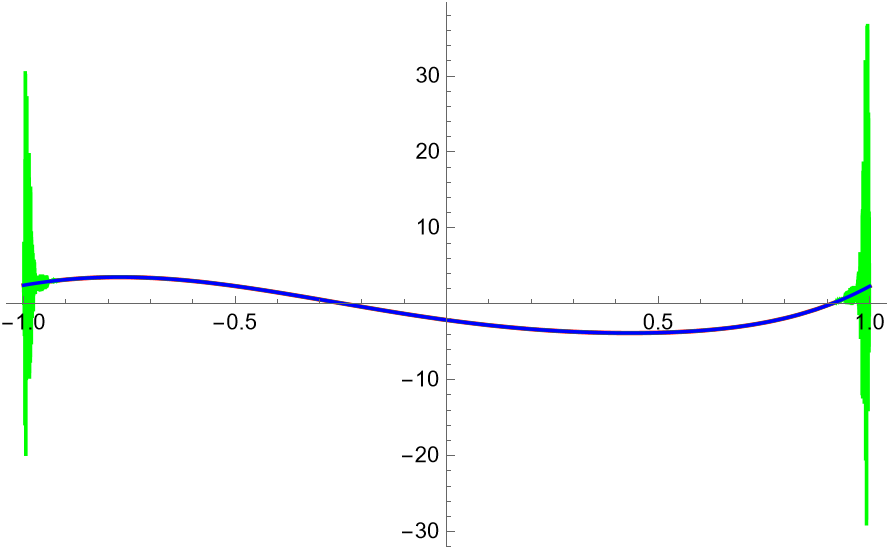
\includegraphics[width=\textwidth]{4_l64}
			\caption{Интерполяция многочленом Лагранжа}
		\end{subfigure}
		\hfill
		\begin{subfigure}{0.4\textwidth}
			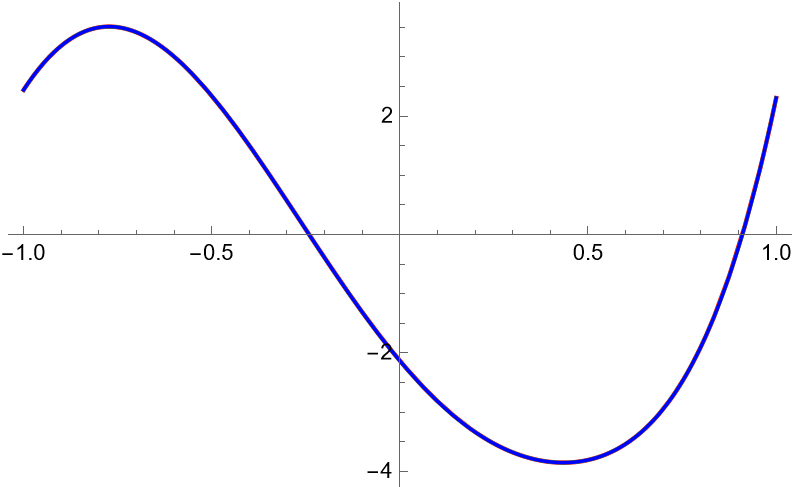
\includegraphics[width=\textwidth]{4_s64}
			\caption{Сплайн-интерполяция}
		\end{subfigure}
		\hfill
		\\[0.5cm]
		\caption{$n = 4$.}
	\end{figure}
	
	
	\newpage
	\begin{thebibliography}{1}
		\bibitem{galanin} \textit{Галанин М.П., Савенков Е.Б.} Методы численного анализа математических\\ моделей. М.: Изд-во МГТУ им. Н.Э. Баумана,	2010. 592 с.
		
		
	\end{thebibliography}
	
	
\end{document}
